\documentclass{deliverablereport}

\usepackage[style=alphabetic,backend=bibtex]{biblatex}
\usepackage{todonotes}
\usepackage{pdfpages}
\addbibresource{report.bib}
\addbibresource{../../lib/publications.bib}

\usepackage{xparse}
\usepackage{etoolbox}
\usepackage{caption}

\deliverable{dissem}{ibook3c}
\duedate{31/07/2019 (M47)}
\deliverydate{31/07/2019}
\author{Hans Fangohr, Thomas Kluyver, Marijan Beg, Min
Ragan-Kelly, Vidar Fauske, Marcin Kostur, Jerzy \L{}uczka
 }

\begin{document}
\maketitle
\githubissuedescription
\newpage
\tableofcontents
\newpage


\section{Reducing barriers for learners and teachers using interactive textbooks}

\subsection{Learners perspective}

The \Jupyter notebook as a virtual research environment holds great
potential for the creation and use of interactive documents. In this
context, we investigate and prototype the use of such interactive
notebooks in the context of education at the university level.

There is a long history in academia to provide textbooks either as
the main point of reference for a given lecture course, or as an
additional "background reading" to provide more details which cannot
be covered by blackboard- or slide-centered lectures, typically due to
the lack of time available.

While providing potentially a wealth of information, such textbooks
are static, and require unusual skill to be exclusively learned
from. Instead, it is a common model to ask students to carry out
practical problem-solving exercises: this enforces engagement with the
material and supports deep learning of the subject.

For computational problems, there is often significant effort required
to set up an environment of software (such as Python with required
libraries or a symbolic mathematics package) and then to set up a
problem environment that allows the study of the topic under
investigation. For example, to solve a differential equation
numerically, the problem environment includes setting up functions
describing the ODE, boundary conditions, and a grid on which the
numerical solution should be obtained. Once this point is reached, the
student can start to explore -- for example -- the properties of a
numerical method being used to solve differential equations.

The \emph{interactive textbooks} developed here allow to improve the
learning experience by significantly reducing this barrier: both
setting up the software environment and setting up the problem
environment are reduced to the task of opening the interactive
document in a browser for which the teacher provides the URL. A short
wait while the virtual environment is created on the fly (using the
Binder service) and navigating to the point of interest in the
textbook. Immediately, it is possible for the learner, to
interactively explore the topic of learning within a prepared learning
and software environment.



\subsection{Teachers perspective}

The easy way to author the manuscript is a key to wide application of
any good practice described in this report. It seems to be easier when
subject is directly connected to computer science. It is natural to
expect that academic teacher lecturing computations is fluent in all
kinds of computer technology. It might not be true, if the subject is
theoretical mechanics or dynamical systems. It can often happen that
such subjects are not integrated with computer technologies during
teaching at all, mostly due to technical or technological barriers.


University of Silesia has experimented to introduce \Sage into science
education in 2011. Initially, the \texttt{sagenb} notebook server was
used as to serve both as computational resources as well as course
material distribution center. Despite its clear limitations, its has
been widely adopted and was used in many courses. In its peak load it
was serving on average one computation per second to 2000 registered
students. The number of created by students notebooks exceeded
20000. Many academic teachers appreciated the fact that our 'cloud'
installation requires merely to login in order to start working. This
feature of the central sagenb turned out to be so important, it had to
be preserved when developing a new solution

As \texttt{sagenb} software became depreciated, there was a
need to find a viable replacement, optimally more flexible which would
allow for application for not only physics and mathematics students
but also useful for e.g. computer science students. \Jupyter
ecosystem with versatile tools and use cases has became an obvious
choice. There where many questions addressed about both ways to
convert old materials, as well as about finding an optimal way to use
those tools in practice. 

During four years of this project we have experimented with many
different ways to effectively create and distribute materials. The
most convenient way of authoring and experimenting at the same time
was writing \Jupyter notebook. This worked equally well for both \Sage
as \Python based materials. Creation of structured document can be
made in many ways. In \longdelivref{dissem}{ibook1} we have explored
application of sphinx system. It has clear advantage of very high
quality output to html and pdf. We managed to implement embedded
sagecell for interactivity of html version. The major disadvantage is,
however, a not negligible barrier for authors. They have to learn
``yet another`` authoring tool and need to have some minimal fluency
in ICT to be able to perform edit-compile-view cycle. In this case the
superior flexibility of sphinx system was sacrificed for simplicity of
\texttt{bookbook} solution. In this approach the only document which
needs to be edited by the author is a \Jupyter notebook. Moreover, the
same workspace, which is used for prototyping and development of the
exercise of example, can be used as initial version of the manuscript.

All technologies developed in this work-package can be transferred to
the European Open Science Cloud in fairly straightforward manner, as
the communication protocol is HTTPS, and all data is written in
structured machine-readable formats.


In the following, we detail the work on the interactive textbooks:
``Computational Science and Engineering'' (Sec.~\ref{sec:computational-science-and-engineering})
and ``Problems in Physics with \Sage'' (Sec.~\ref{seq:problems-in-physics})



\todo[inline]{Viviane/Nicolas, please update as required.}

\section{Interactive text book on Computational Science and Engineering}
\label{sec:computational-science-and-engineering}

\subsection{Context and overview}


The application of mathematics in science and engineering is the topic
of the textbook "Introduction to Python Computational Science and
Engineering".
%
The target audience is scientists outside computer science. It is
thus important to teach some programming basics before using those to
conduct computational and data science tasks.

The work is based on a textbook that was available as a PDF file (and
generated from a \LaTeX{} file). In this deliverable, we have reviewed
the textbook and updated it from Python 2 to Python 3, added various
sections and a chapter on Pandas, but most importantly translated the
\LaTeX{} sources into \Jupyter notebooks. Furthermore, we used and
evaluated tools such as \texttt{bookbook} and \texttt{nbconvert} to
automatically convert the textbook in alternative formats.

The new PDF is created from the \Jupyter notebooks by auto-generating
\LaTeX{} sources compiling them to create a high quality PDF file. A
\LaTeX{} file with custom style settings can be given as a template to
the \texttt{bookbook} package. The different chapters (each being one
notebook) are merged automatically, and get a joint table of contents.

From the same \Jupyter notebook sources, a set of HTML files can be
created to allow more convenient online reading of the material. These
HTML files are organized into one HTML file per chapter (each being
created from one notebook), and an additional index file providing
links to all chapters.

The (automatic) translation of the \Jupyter notebook-based textbook
into PDF is important to provide (at least) the same level of
publication quality outputs that can be expected from the more
traditional \LaTeX{} based manuscript. The conversion to HTML is an
added bonus, and offers a way of reading the document that is more
appropriate for commonly used devices such as laptops, tablets, and
smart phones.

\TODO{Is thebelab enabled on the HTML version?}

\subsection{Availability}

The complete book is open source and available from\newline
{\tiny\url{https://github.com/fangohr/introduction-to-python-for-computational-science-and-engineering}}\linebreak
under a Creative Commons license (Attribution-NonCommercial 4.0
International (CC BY-NC 4.0)).

A Zenodo entry has been created (\url{https://doi.org/10.5281/zenodo.1411868}).

\subsection{Uptake and feedback}

The textbook is used regularly at the University of Southampton to
teach all engineering students about computational science in their
first year of studies (typical numbers of students per year between
300 and 500). The physics department has also started to adapt these
materials. Due to Prof. Fangohr's move to European XFEL and the
University of Hamburg, the textbook is also in use in optional
courses at the Physics department to provide an introduction to
computational science.

We know from instructors at other institutions that they are using the
textbook in their teaching, including Aalborg University (Denmark),
Haverford College (Pennsylvania, US), Tulane University, New Orleans
(US), GeorgiaTech, Georgia (US), University of California, Santa Cruz,
California (US), University of South California, Los Angeles
(US), Federal University of Paraiba, Paraiba (Brasil), University of
Virgin Islands, Virgin Islands (US). These courses are typically
outside computer science and addressing engineers, biologists,
meterologists, chemists etc.

We have also heard from individual students that participate in other
courses at universities or courses from Coursera and who have enjoyed
the textbook as a freely available complement, providing static and
interactive learning material.

A translation into Portuguese is available, including the interactive
version on Binder.\footnote{https://github.com/gcpeixoto/lecture-ipynb/blob/master/README.md}
\pagebreak


\section{Interactive text books: Problems in Physics with SageMath}
\label{seq:problems-in-physics}


\subsection{Context and overview}

Problems in Physics with \Sage is a set of lecture notes collected for
over one decade during teaching activities at University of
Silesia. Topics range from classical mechanics to dynamical systems
and transport processes. Those materials have been used for teaching
in following courses: Theoretical Mechanics, Introduction to fluid
dynamics, Programming massively parallel processors in CUDA,
Mathematical Methods in Biophysics.


At the University of Silesia (Institute of Physics), the content of
the material in the e-books has been exploited for many years as parts
of lectures and exercises for two groups of students: the second year
of study of biophysics (Mathematical Methods of Biophysics) and the
fourth and fifth year of physics study (seminars and monograph
lectures). In summary, about 100 students participated in the above
courses. From our experience it follows that in particular it has been
useful for students of biophysics who are less fluent in calculations
and transformations of mathematical expressions. The possibility of
graphical presentation allows them to acquire intuition and better
understanding of properties and behavior of some processes and
phenomena.

\subsection{Availability}

The complete book consists of three parts and are  open source and available from:\newline
{\url{https://github.com/marcinofulus/Mechanics_with_SageMath}\linebreak
{\url{https://github.com/marcinofulus/Dynamical_Systems}\linebreak
{\url{https://github.com/marcinofulus/Transport_Processes}\linebreak
under a Creative Commons license (Attribution-NonCommercial 4.0
International (CC BY-NC 4.0)).

\subsection{Part I: Classical Mechanics with \Sage}

This book contains set of problems solved with the help of computer
algebra. It consists of \Jupyter notebooks with \Sage kernel.
\todo{to be finished!}

\subsection{Part II: Dynamical Systems}

The interactive book "Dynamical Systems" has its source in teaching
students of Econophysics at the Faculty of Mathematics, Physics and
Chemistry (University of Silesia). Next, the content of this course
has been extended to students of theoretical physics and
biophysics. This course is very attractive for using Sage. Applying
Sage, it shows that analysis of some classes of dynamical systems (as
a set of differential equations) is much more simpler and it allows to
understand even complicated behavior of processes appearing in natural
sciences.  This course starts with motivation of using differential
equations for modeling of some processes in physics, biophysics and
econophysics. Fundamental information on a set of autonomous
differential equations is presented with minimal mathematical
apparatus. Very impressive are examples showing non-uniqueness of
their solutions. Elementary notions like phase space, phase curves and
vector fields associated with differential equations are introduced
and examples are shown by using Sage. The next section of the e-book
concerns attractors. Again, various classes of attractors can be
presented for differential equations by applying Sage. In classical
mechanics, conservative and dissipative systems play a crucial role in
understanding statistical physics, irreversible processes and chaotic
properties of deterministic systems. It is a subject of one of the
section. The final part of the book is devoted to a difficult notion
of deterministic chaos. As an example, we consider a classical
particle moving in a bistable potential and driven by a time periodic
force. In this part, Sage appears to be extremely useful in visual
demonstration and understanding of chaotic properties of relatively
simple dynamical systems. Without Sage it would be impossible to apply
any analytical and tractable methods to obtain desired information on
this system.


\subsection{Part III: Transport Processes}

The interactive book ``Transport Processes'' is based on two courses
taught in Institute of Physics at University of Silesia: Introduction
to fluid dynamics, Programming massively parallel processors in
CUDA. Those courses were intended for graduate students and PhD
students. In both courses we followed problem oriented
teaching. Student were given a \Jupyter notebook with introductory
information and the problem statement. After some time of individual
work solution were returned. In this cases grading was performed
manually, usually followed by discussion of problems and methods of
solution individually with a student.

\subsection{Outlook and future work}

A new academic year 2019/2020 starts with the new and big Faculty of
Natural Sciences and Technology. Therefore the e-books will be used
for wider audience of students, not only in physics but also in
material sciences and computer sciences. Our colleagues from other
Polish higher schools are also interested in using the presented
e-books.


\section{Authoring and using interactive textbooks}

\subsection{Added value of the Notebook based textbook}

The additional value comes from the \Jupyter Notebook based
nature of the chapters:

\begin{enumerate}
\item Students can download the notebooks and inspect all the
  computational steps that have created the results shown in the
  textbook. Assuming they have the relevant software installed,
  they can execute them on their own machine, modify,
  explore, understand, and extend the examples. As all computational
  steps are included in the notebooks, there is no guessing about
  assumptions, no code being executed before an example is introduced,
  or no reconstructions of sections labeled ``the required
  transformation of X is left as an exercise to the reader'' required:
  all steps are contained in the notebooks. This reduces the barrier
  towards learning.

\item
  Using the cloud hosted \texttt{Binder} service
  (\url{http://mybinder.org}), learners can open the book in an
  temporary \emph{Virtual Research Environment (VRE)} that has been
  created on demand just for them. While providing all the advantages
  outlined above, in this setup \emph{no software installation is
    required}.

  In more detail in the case of ``Introduction to Python Computational Science and Engineering'':

  The textbook can come with a specification of the software it
  requires (for example through a Python \texttt{requirements.txt}
  file). For the textbook at hand that specification is
  straightforward: indeed it requires no software beyond the standard
  scientific Python stack (numpy, scipy, matplotlib, pandas, \Jupyter,
  ...) which is included in the default Anaconda Python distribution.

  The textbooks and specification can be referenced by a URL. When a
  student accesses this URL with his browser, the \texttt{Binder}
  constructs on demand a Docker image including a copy of the
  notebooks and the required software, and provisions a temporary
  Docker container (lightweight virtual machine) running a \Jupyter
  notebook server. The student can browse through the textbook, and
  execute chapter notebooks as they like to achieve better
  understanding.
\end{enumerate}

\subsection{Good practice in software engineering for
  computational science [textbooks]}\label{sec:good-pract-softw}

We have used the following technologies and processes to improve the
quality and maintainability of the open source textbook:
\begin{itemize}
  
\item The sources are available and publicly readable on
  Github\footnote{https://github.com/fangohr/introduction-to-python-for-computational-science-and-engineering}
\item Changes in the files are tracked through commits in Git.
\item Together with the executable textbooks, we have defined
  \emph{automatic tests} that can re-execute all material in the
  notebook to check that reported outputs are produced by the
  displayed inputs.

  This uses the \nbval tool -- developed as part of OpenDreamKit -- to
  re-execute the chapters, and to compare the computed output with the
  output that is stored with the notebook.

  If deviations or even exceptions arise, then the displayed example
  output is not generated from the computational input, and thus the
  chapter is outdated (or simply wrong). For conventional
  (non-interactive) textbooks, such gradually becoming outdated is
  hard to recognize, and typically updated with the next edition a
  few years later.

  In the context of this textbook, there are two common sources for
  deviations reported by \nbval:
  \begin{enumerate}
  \item Changes in the chapter have had (unexpected) side effects
    later in the chapter, combined with a failure to re-execute the
    whole chapter manually to check for such deviations after the
    changes were introduced.
  \item Changes in libraries we depend on: for example, the change to
    Matplotlib version 3 has introduced new behaviour of Matplotlib,
    which resulted in different outputs.
  \end{enumerate}

\item These automatic tests are executed whenever changes are
  committed to the repository, or when a branch is requested to be
  merged into the master branch. We use Travis CI for this, which
  provides this service free of charge for open repositories\footnote{
  https://travis-ci.org/fangohr/introduction-to-python-for-computational-science-and-engineering}

  This makes it feasible to consider community contributions to the
  textbook: at least the internal consistency of input and output for
  any contribution is checked automatically, even before the author
  team starts reviewing the proposed changes or additions.

\item We use (Docker) containers on the Travis CI testing system to
  host the software environment within which the notebooks are
  executed and converted to generate the PDF and HTML version, and we
  also use this container environment to compare input and outputs
  (using NBVAL, see above).

  Using containers here has the following advantages:
  \begin{enumerate}
  \item Through the \texttt{Dockerfile} (and the \texttt{.travis.yml}
    file), the building of the container is fully defined: users who
    want to also convert the notebooks to HTML or PDF, or re-recreate
    what is done on the continuous integration system, can either
    create the same container, or follow the installation on a virtual
    machine or bare metal machine. In any case, having these
    configurations available is more explicit than using the default
    Linux and configuration that Travis CI provides.

  \item If a problem arises in the continuous integration, we can
    replicate the same environment locally (in a Docker container on
    our own workstation/laptop) and fix it there: this is more
    effective than having to commit to the repository and to wait for
    Travis CI to re-execute the tests to check if the problem has
    disappeared.

  \end{enumerate}

%\newpage\printbibliography
\end{itemize}

\subsection{Integration into MyBinder}

The following  textbooks are available through MyBinder service: on the github webpage of the
books link to the MyBinder service is provided.

\begin{itemize}
\item ``Introduction to Python for Computational Science and Engineering''\footnote{https://github.com/fangohr/introduction-to-python-for-computational-science-and-engineering/blob/master/Readme.md}
\item ``Mechanics with \Sage''\footnote{https://github.com/marcinofulus/Mechanics\_with\_SageMath/blob/master/README.md}
\end{itemize}

By clicking on it, the user is served a computational environment in
the cloud in which the textbook can be read, engaged with, and
interactively executed.

Additional links are provided to launch the notebooks in a JupyterLab
(rather than the classic \Jupyter Notebook) environment.

At the moment, this service is supported by funds from the \Jupyter
Project, but given ongoing development for the Binder project, and
interest from the European Open Science Cloud and various universities
and research facilities, it is likely that other MyBinder services
appear which can be used for such interactive document hosting in the
future. Of course there is a question over how this is financed -- one
possibility would be to finance this from overheads; comparable to
library costs and access to the Internet that are already accepted as
overheads in research and education.

Technically, we have specified our software requirements through a
\texttt{requirements.txt} file in the root of the repository. This is
the preferred way for Binder to read the specification, and also good
because we can express software requirements for execution of the
notebooks (which are relevant to learners) in this human readable
file.

When we build the container for the continuous integration (see
Sec.~\ref{sec:good-pract-softw}), we use a \texttt{Dockerfile} in a subdirectory
\texttt{docker/} (so that Binder does not see this file as it would
override the requirements provided in \texttt{requirements.txt}), and
when building the Docker image, we pip-install all dependencies listed
in the \texttt{requirements.txt} file. We thus eliminate duplication
of requirements completely.



\pagebreak
\appendix
\section{Appendix 1: Table of contents of the interactive book}\label{sec:appendix-1}

On the following 5 pages, we show the table of contents of the
interactive book \emph{Introduction to Python for Computational
  Science and Engineering}.
%
The full materials are available at
\newline
https://github.com/fangohr/introduction-to-python-for-computational-science-and-engineering

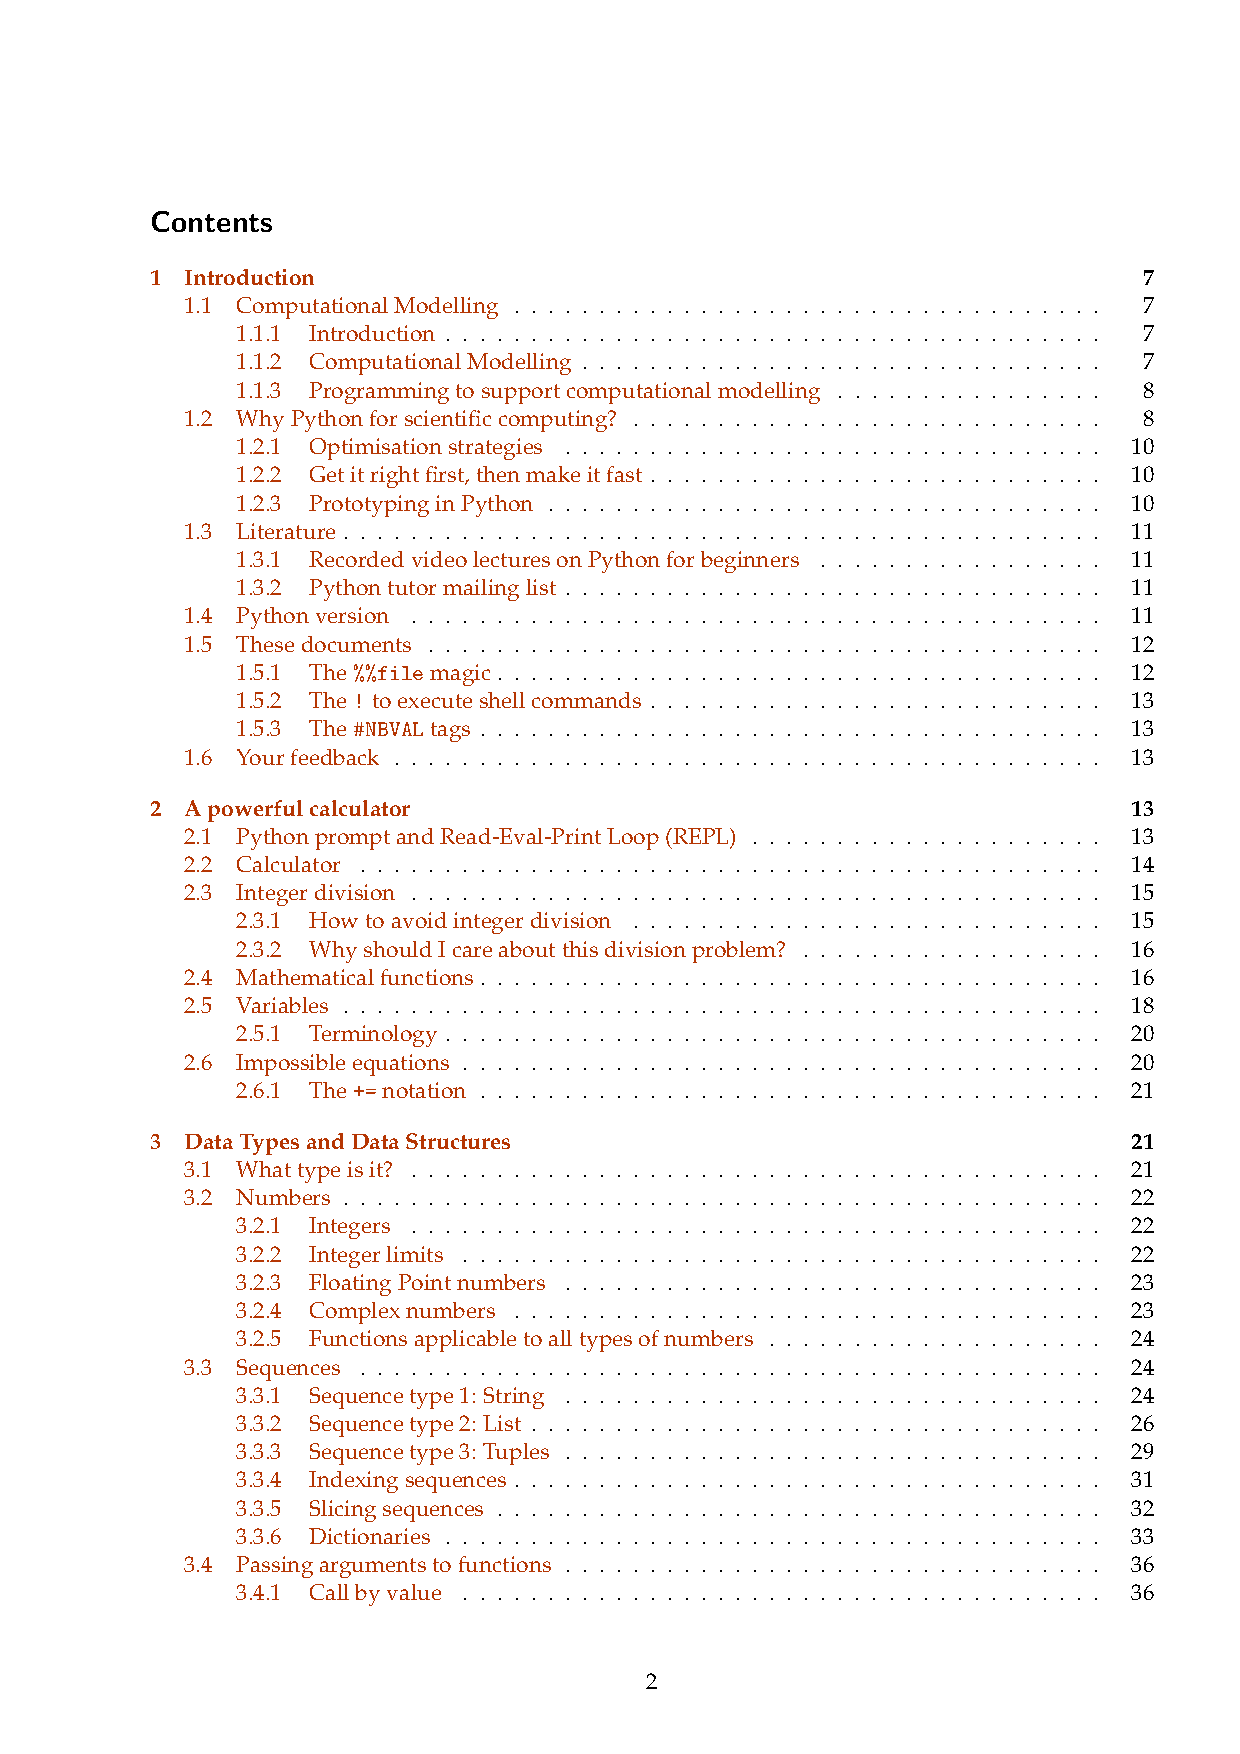
\includepdf[pages={1-5}]{computational-science-table-of-contents.pdf}



\section{Appendix 2: Table of contents of the interactive book}\label{sec:appendix-1}

On the following 5 pages, we show the table of contents of the
interactive book \emph{Mechanics with \Sage}.
%
The full materials are available at
\newline
https://github.com/marcinofulus/Mechanics\_with\_SageMath
\includepdf[pages={2-4}]{mechanics_with_sagemath_toc.pdf}


\end{document}

%%% Local Variables:
%%% mode: latex
%%% TeX-master: t
%%% End:
